\section{EGMN model (Q\&A)}

\subsection{Q: What is EGMN in this repository?}
\noindent\textbf{A:} EGMN (Exponential--Gaussian Mixture Network), implemented in \lstinline|model/egmn.py|, predicts watch time by modeling a \textbf{mixture distribution} that captures short ``quick-skip'' behavior and longer watch-time behavior.

\subsection{Q: What distribution family does EGMN use?}
\noindent\textbf{A:} EGMN uses a mixture consisting of \(1\times\) Exponential (short peak near 0) plus \(K\times\) Gaussian components for longer watches, implemented as Normals truncated below at 0, i.e. \(p(y)=\pi_0\,\mathrm{Exp}(y;\lambda)+\sum_{k=1}^{K}\pi_k\,\mathrm{TN}(y;\mu_k,\sigma_k,\text{lower}=0)\) for \(y\ge 0\).

\subsection{Q: What does the architecture look like end-to-end?}
\noindent\textbf{A:} The model encodes sparse/sequence/continuous features into a shared representation, feeds it through a shared MLP trunk, and uses separate heads to produce \(\pi\) logits, \(\lambda\), \(\mu\), and \(\sigma\), which parameterize the mixture used for training and prediction.
\begin{figure}[h]
  \centering
  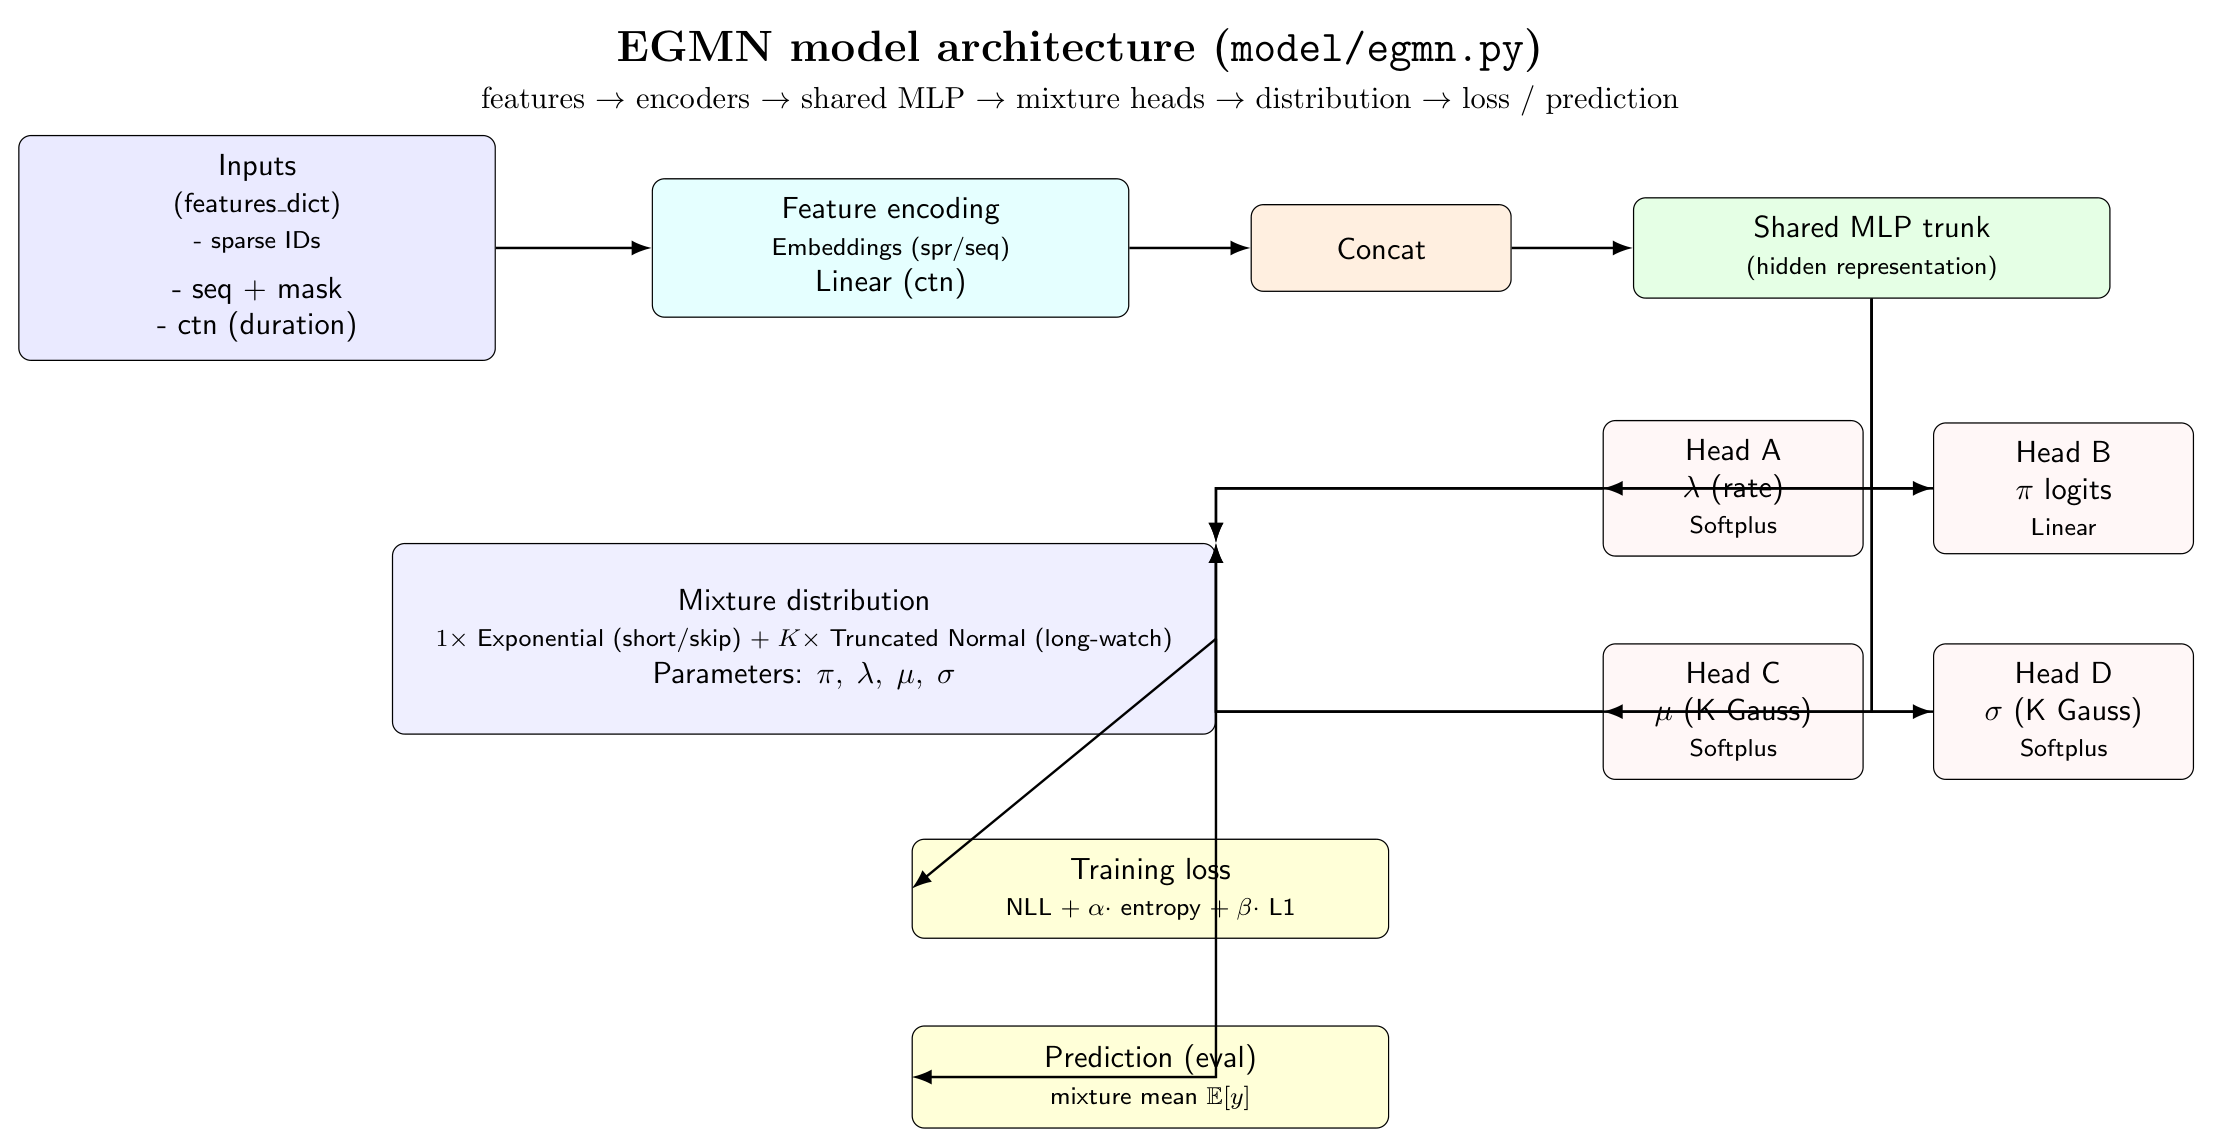
\includegraphics[width=\textwidth]{figures/egmn_arch.png}
  \caption{EGMN architecture overview: feature encoders + shared MLP + mixture-parameter heads, producing a distribution and a mean prediction.}
\end{figure}

\subsection{Q: What parameters (heads) does EGMN output in code?}
\noindent\textbf{A:}
\begin{lstlisting}[language=Python]
# model/egmn.py (illustrative excerpt)
self.lambda_layer = nn.Sequential(
    nn.Linear(hidden_dim, 1),
    nn.Softplus(beta=0.5),
)

comp_num = 10  # number of Gaussian components
self.mixture_logits = nn.Linear(hidden_dim, comp_num + 1)  # +1 for Exponential
self.gauss_mu = nn.Sequential(nn.Linear(hidden_dim, comp_num), nn.Softplus())
self.gauss_sigma = nn.Sequential(nn.Linear(hidden_dim, comp_num), nn.Softplus())
\end{lstlisting}

\subsection{Q: What loss does EGMN train with in the run script?}
\noindent\textbf{A:} Training minimizes a mixture negative log-likelihood plus regularizers: \(\mathcal{L}=\mathcal{L}_{\mathrm{NLL}}+\alpha\,\mathcal{L}_{\mathrm{entropy}}+\beta\,\mathcal{L}_{\mathrm{reg}}\), where \(\mathcal{L}_{\mathrm{reg}}\) is an L1 reconstruction between label and mixture-mean prediction and \(\mathcal{L}_{\mathrm{entropy}}\) is a mixture-weight entropy term.

\subsection{Q: What scalar output is used for evaluation?}
\noindent\textbf{A:} The evaluation uses a point estimate equal to the \textbf{mixture mean} (including the exponential mean \(1/\lambda\)), producing one scalar prediction per example.

\subsection{Q: How is the mixture-mean prediction computed (schematically)?}
\noindent\textbf{A:}
\begin{lstlisting}[language=Python]
# model/egmn.py (illustrative excerpt)
pi, lambda_, mu, sigma = self.forward(features)
pi = torch.softmax(pi, dim=1)
component_means = torch.concat([1 / lambda_, mu], dim=1)
pred = torch.sum(pi * component_means, dim=1)
\end{lstlisting}
